\documentclass{article}

\usepackage{float}
\usepackage{graphicx}

\title{Performance Analysis of GPU-Accelerated Optical Flow}
\date{December 8, 2014}
\author{Hari Caushik, Kyle Cesare, Soo-Hyun Yoo}

\begin{document}

\maketitle

\newpage

\tableofcontents

\newpage

\section{Introduction}
This is just a test.

\section{Testing Methodology}
To test the criteria outlined above, we will create two programs to produce
identical outputs, but one will target a CPU and the other a GPU.

To try to identify strengths and weaknesses of each target, we will attempt to
introduce additional variables that may have an impact on performance. These
variables will be:

\begin{description}
  \item[Image resolution] To process a very small image, the overhead required
    to copy memory between the CPU and GPU may be larger than the actual
    processing time. We will use video at QVGA (320x240), VGA (640x480) and FHD
    (1920x1080) to see if this effect is significant.
  \item[Flow magnitude] ?
\end{description}

It is important to note that the processing times for the first few frames will
be discarded to remove any caching oddities and to allow the GPU kernels to
finish load.

\section{Results}

\begin{figure}[H]
  \centering
    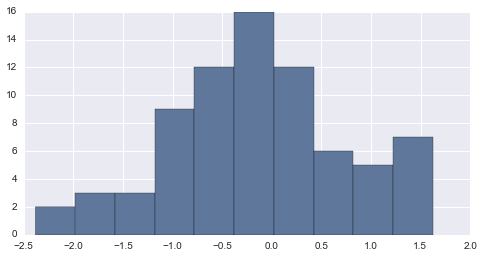
\includegraphics[width=0.8\textwidth]{test_resolution.png}
  \caption{Processing time per frame at various resolutions.}
\end{figure}

\begin{figure}[H]
  \centering
    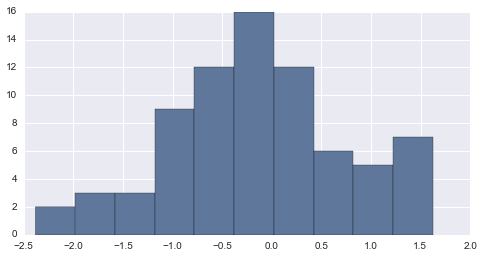
\includegraphics[width=0.8\textwidth]{test_flow.png}
  \caption{Processing time per frame for various magnitudes of motion.}
\end{figure}

\section{Implementation Analysis}
To provide more insight into why the GPU showed better performance results than
the CPU, we will now break down the OpenCV Farneback optical flow implementation
used in the trials. We use the \texttt{objdump} tool to disassemble the OpenCV
shared library into an x86 assembly representation. We then use this assembly
code to gather information on the types and counts of instructions being run.

The heavy use of Streaming SIMD Extensions (SSE) makes it more difficult to
reason about the number of floating point operations being performed.

\section{Conclusion}

\end{document}
